\documentclass[11pt]{article}
\usepackage{amsmath}
\usepackage{amssymb}
\usepackage{minted}
\usepackage{graphicx}
\usepackage{bbm}
\usepackage{float}
\usepackage[margin=0.5in,footskip=0.25in]{geometry}

\setlength{\textwidth}{6.5in}
\setlength{\oddsidemargin}{0.0in}
\setlength{\textheight}{9.0in}
\setlength{\parindent}{0in}

\newcommand{\problem}[1]{ \medskip \pp $\underline{\rm Problem\ #1}$\\ }

\def\pp{\par\noindent}
\DeclareMathOperator{\E}{\mathbb{E}}
\begin{document}

\centerline{\{\bf Amy Qi, xq2224\}}
\centerline{\bf Homework 4 Solutions}
\centerline{\bf W4771 Machine Learning --- Fall 2023}

\bigskip 
\bigskip

\section*{Problem 1}
To check whether a function is positive definite is essentially checking if the matrix
\[ K = 
\begin{bmatrix}
    k(x^{(1)}, x^{(1)}) & \ldots & k(x^{(1)}, x^{(n)})\\
    \vdots & \ddots & \vdots \\
    k(x^{(n)}, x^{(1)}) & \ldots & k(x^{(n)}, x^{(n)})
\end{bmatrix}
\]
is positive semi-definite, i.e., for any vector $x \in \mathbb{R}^n$, $x^T K x \geq 0$.

\subsection*{(a)}
NOT NECESSARILY POSITIVE DEFINITE \\
Adding each entry of the matrix by 2 is the same as adding a matrix that is all 2 of the same dimension to $K$. Thus $x^T K_a x = x^T (K + K_{all 2}) x $, which might not be non-negative for all x.

\subsection*{(b)}
POSITIVE DEFINITE \\
Scaling a positive semi-definite matrix by a positive scalar results in a positive semi-definite matrix, i.e., $x^T K_b x = 2x^T K x \geq 0$.

\subsection*{(c)}
POSITIVE DEFINITE \\
Adding to positive semi-definite matrices result in a positive semi-definite matrix. $x^T K_c x = x^T (K+\widetilde{K}) x = x^T K x + x^T \widetilde{K} x$. Since both $x^T K x$ and $x^T \widetilde{K} x$ are greater than or equal to 0, their sum should also be greater than or equal to 0. Thus $x^T K_c x \geq 0$.

\subsection*{(d)}
NOT NECESSARILY POSITIVE DEFINITE \\
$x^T K_c x = x^T (K-\widetilde{K}) x = x^T K x - x^T \widetilde{K} x$. Since it might be possible that for some $x$, $x^T K x < x^T \widetilde{K} x$, matrix $K_c$ is not necessarily positive definite.

\subsection*{(e)}
POSITIVE DEFINITE\\
According to the Schur product theorem, the Hadamard product of two positive semi-definite matrices is also positive semi-definite. Substituting $k_e(x,z) = k(x,z) \cdot \Tilde{k}(x,z)$, each entry in the new matrix is the Hadamard product of $K$ and $\widetilde{K}$, so this matrix is positive semi-definite as well.


\section*{Problem 2}
\begin{equation}
    \begin{split}
        \text{LHS} & =(A^TA+\lambda I)^{-1}A^T \\
        &= (A^TA+\lambda I)^{-1} \cdot A^T \cdot I \\
        &= (A^TA+\lambda I)^{-1} \cdot A^T (AA^T + \lambda I) \cdot (AA^T + \lambda I)^{-1} \\
        &= (A^TA+\lambda I)^{-1} \cdot (A^TAA^T + A^T\lambda I) \cdot (AA^T + \lambda I)^{-1} \\
        &= (A^TA+\lambda I)^{-1} \cdot (A^TA + \lambda I) \cdot A^T \cdot (AA^T + \lambda I)^{-1} \\
        &= A^T \cdot (AA^T + \lambda I)^{-1} = \text{RHS}
    \end{split}
\end{equation}

\section*{Problem 3}
\subsection*{(a)}
To show that k is a positive definite kernel, we want to show that $\sum_{i=0}^n \sum_{j=0}^n c_i c_j k(x_i, x_j)\geq 0$ for any $x_1\ldots x_n$ and $c_i \ldots c_n$. This is shown below. \\

\begin{equation}
    \begin{split}
        \sum_{i=0}^n \sum_{j=0}^n c_i c_j min\{x_i, x_j\} &= \sum_{i=0}^n \sum_{j=0}^n c_i c_j \int_{0}^{\infty}{\mathbbm{1}\{t\leq min\{x,z\}\} \, dt} \\
        &= \sum_{i=0}^n \sum_{j=0}^n c_i c_j \int_{0}^{\infty}{\mathbbm{1}\{t\leq x_i\} \mathbbm{1}\{t\leq x_j\} \, dt} \\
        &= \int_{0}^{\infty}{ \sum_{i,j=0}^n c_i c_j \mathbbm{1}\{t\leq x_i\} \mathbbm{1}\{t\leq x_j\} \, dt} \\
        &= \int_{0}^{\infty}{ \sum_{i=0}^n (m_i \cdot \mathbbm{1}\{t\leq x_i\})^2 \, dt} \\
        &\geq 0
    \end{split}
\end{equation}
Justification for the last step: if we expand the squares then it can be discovered that all combinations of $\mathbbm{1}\{t\leq x_i\} \mathbbm{1}\{t\leq x_j\}$ are there.

\subsection*{(b)}
The optimal value for $\lambda$ is $0.25$. The test mean square error using this value is $0.10949523552572395$. \\
The plot is shown below. \\
\begin{figure}[H]
    \centering
    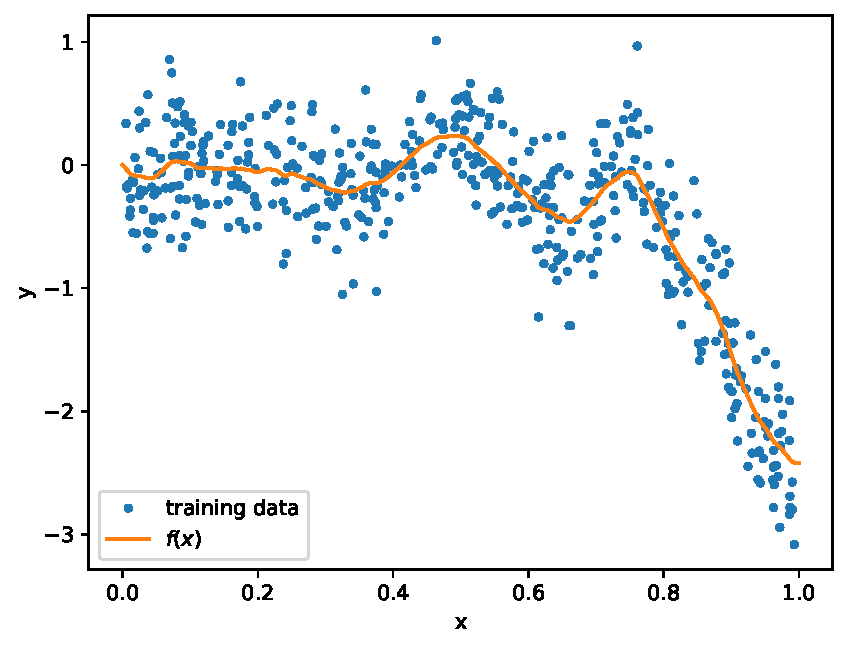
\includegraphics[scale=0.8]{images/hw4reg.pdf}
\end{figure}

\subsection*{(c)}
The values I use for part (c) are $\lambda = 1$ and $\sigma = 0.1$. The $\lambda$ values are chosen from $\{0.1,0.2, \ldots 0.9,1\}$.
 The test mean square error using this value is $0.11431527284842233$. \\
The plot is shown below. \\
\begin{figure}[H]
    \centering
    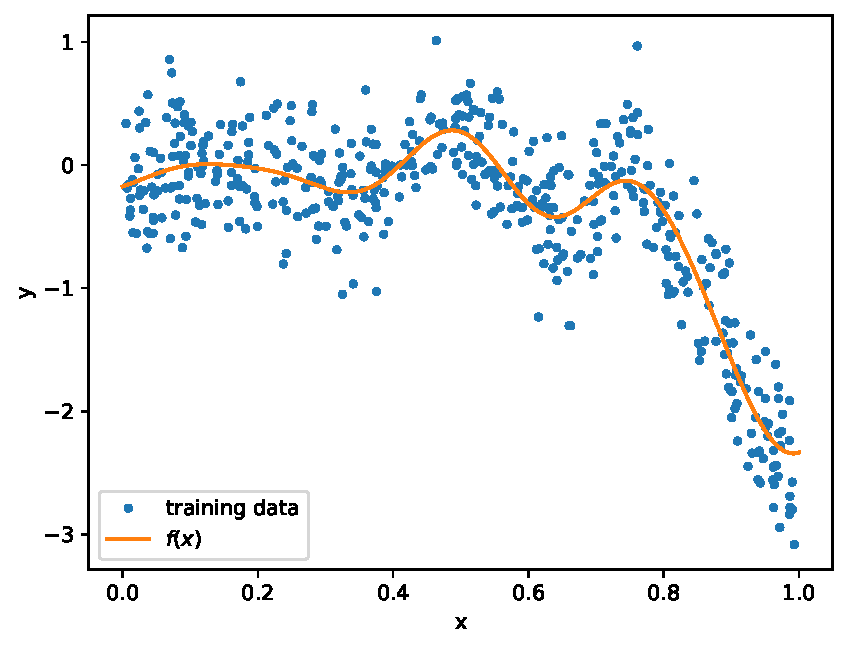
\includegraphics[scale=0.8]{images/hw4regc.pdf}
\end{figure}

\section*{Problem 4}
\subsection*{(a)}
TRUE\\

Since gain(span$\{q_1,q_2\}$) $=||Aq_1||^2+||Aq_2||^2$ and gain(span$\{v_1,v_2\}$) $=\sigma_1^2 + \sigma_2^2$, to show that $||Aq_1||^2+||Aq_2||^2 = \sigma_1^2 + \sigma_2^2$, we only need to show gain(span$\{q_1,q_2\}$) $=$ gain(span$\{v_1,v_2\}$). To show this, we will prove below that span$\{q_1,q_2\}$ $=$ span$\{v_1,v_2\}$. \\

First we show that $\text{span}\{q_1,q_2\} \subseteq \text{span}\{v_1,v_2\}$. \\
% To show this, consider $Aq_1$. Substitute the formula for singular value decomposition into this expression, we have $\sum_{i=1}^r \sigma_i u_i v_i^Tq_1$. Similarly for $A_q2$, we have $\sum_{i=1}^r \sigma_i u_i v_i^Tq_2$. 
Since span$\{Aq_1,Aq_2\}$ $=$ span$\{u_1,u_2\}$, we can write $Aq_1$ as a linear combination of $u_1$ and $u_2$. Since $u_1$ is what we get from the singular decomposition of $A$, we know $u_i = 1/\sigma_1 \cdot A v_1$. Substituting that into the equation, $Aq_1 = m Au_1 + nAu_2 = A (mu_1 + nu_2)$, which indicates that for any given $q_1$, we can express it as a linear combination of $u_1$ and $u_2$. Similarly we can argue for any given $q_2$, we can express it as a linear combination of $u_1$ and $u_2$. Therefore $\text{span}\{q_1,q_2\} \subseteq \text{span}\{v_1,v_2\}$. \\ 

% we know that for $i\geq 3$, $\sigma_i u_i v_i^Tq_1 = 0$. Since the singular values are greater than 0, we know the inner product $<v_i, q1>$ and $<v_i, q2>$ are all zeros for $i\geq 3$. That means neither of $q_1$ or $q_2$ is in the span of $v_i$ for $i\geq 3$. \\

Then we show that $\text{span}\{v_1,v_2\} \subseteq \text{span}\{q_1,q_2\}$. \\
Since span$\{Aq_1,Aq_2\}$ $=$ span$\{u_1,u_2\}$, we know $u_1$ can be written as some linear combinations of $Aq_1,Aq_2$, i.e., $u_1 = m Aq_1 + n Aq_2$. Since $u_1$ is what we get from the singular decomposition of $A$, we know $u_i = 1/\sigma_1 \cdot A v_1$. Substituting that into the equation, $A v_1 = m Aq_1 + n Aq_2 = A (m q_1 + n q_2)$, which indicates that for any given $v_1$, we can express it as a linear combination of $q_1$ and $q_2$. Similarly we can argue for any given $v_2$, we can express it as a linear combination of $q_1$ and $q_2$. Therefore, $\text{span}\{v_1,v_2\} \subseteq \text{span}\{q_1,q_2\}$. \\

Combine the two cases, we know span$\{q_1,q_2\}$ $=$ span$\{v_1,v_2\}$ given span$\{Aq_1,Aq_2\}$ $=$ span$\{u_1,u_2\}$, which indicates that $||Aq_1||^2+||Aq_2||^2 = \sigma_1^2 + \sigma_2^2$, and that the statement is true.

\subsection*{(b)}
FALSE\\

Proof by contradiction. Suppose the statement is true, that if $q_1$ and $q_2$ are orthonormal vectors in $\mathbb{R}^d$ such that $||Aq_1||^2+||Aq_2||^2 = \sigma_1^2 + \sigma_2^2$, then the span$\{Aq_1,Aq_2\}$ $=$ span$\{u_1,u_2\}$. We will show by contradiction that this is not possible given a counterexample when $\sigma_2 = \sigma_3$. \\

Suppose $q_1 = \frac{\sqrt{2}}{2}v_1 + \frac{\sqrt{2}}{2}v_3$, $q_2 = -\frac{\sqrt{2}}{2}v_1 + \frac{\sqrt{2}}{2}v_3$. These two are orthonormal. \\

Thus $Aq_1 = \frac{\sqrt{2}}{2}\sigma_1v_1 + \frac{\sqrt{2}}{2}\sigma_3 v_3$, $Aq_2 = \frac{\sqrt{2}}{2}\sigma_2v_2 + \frac{\sqrt{2}}{2}\sigma_3 v_3$. And we have $||Aq_1||^2+||Aq_2||^2 = \sigma_1^2 + \sigma_3^2 = \sigma_1^2 + \sigma_2^2$. \\

However, $Aq_1 \in \text{span}\{u_1,u_3\} \neq \text{span}\{u_1,u_2\}$, since $u_i$s are orthonormal. That means span$\{Aq_1,Aq_2\}$ $\neq$ span$\{u_1,u_2\}$, and the statement is false.

% If $\sigma_2 = \sigma_3$, $||Aq_1||^2+||Aq_2||^2 = \sigma_1^2 + \sigma_2^2 = \sigma_1^2 + \sigma_3^2$. \\
% Since $||Aq_1||^2+||Aq_2||^2 = \sigma_1^2 + \sigma_2^2$, from our assumption we know span$\{Aq_1,Aq_2\}$ $=$ span$\{u_1,u_2\}$. 
% % And since span$\{Aq_1,Aq_2\}$ $=$ span$\{u_1,u_2\}$, we know that the inner products between $<v_i,q_1>=0$ for all $i \geq 3$. \\
% Similarly, since $||Aq_1||^2+||Aq_2||^2 = \sigma_1^2 + \sigma_3^2$, from our assumption we know span$\{Aq_1,Aq_2\}$ $=$ span$\{u_1,u_3\}$. \\
% That indicates span$\{u_1,u_2\}$ $=$ span$\{u_1,u_3\}$, which cannot be true because $u_i$ for $i \in \{1 \ldots r\}$ are orthonormal. Contradiction. \\
% Therefore, this statement must be false.


\section*{Problem 5}
\begin{figure}[H]
    \centering
    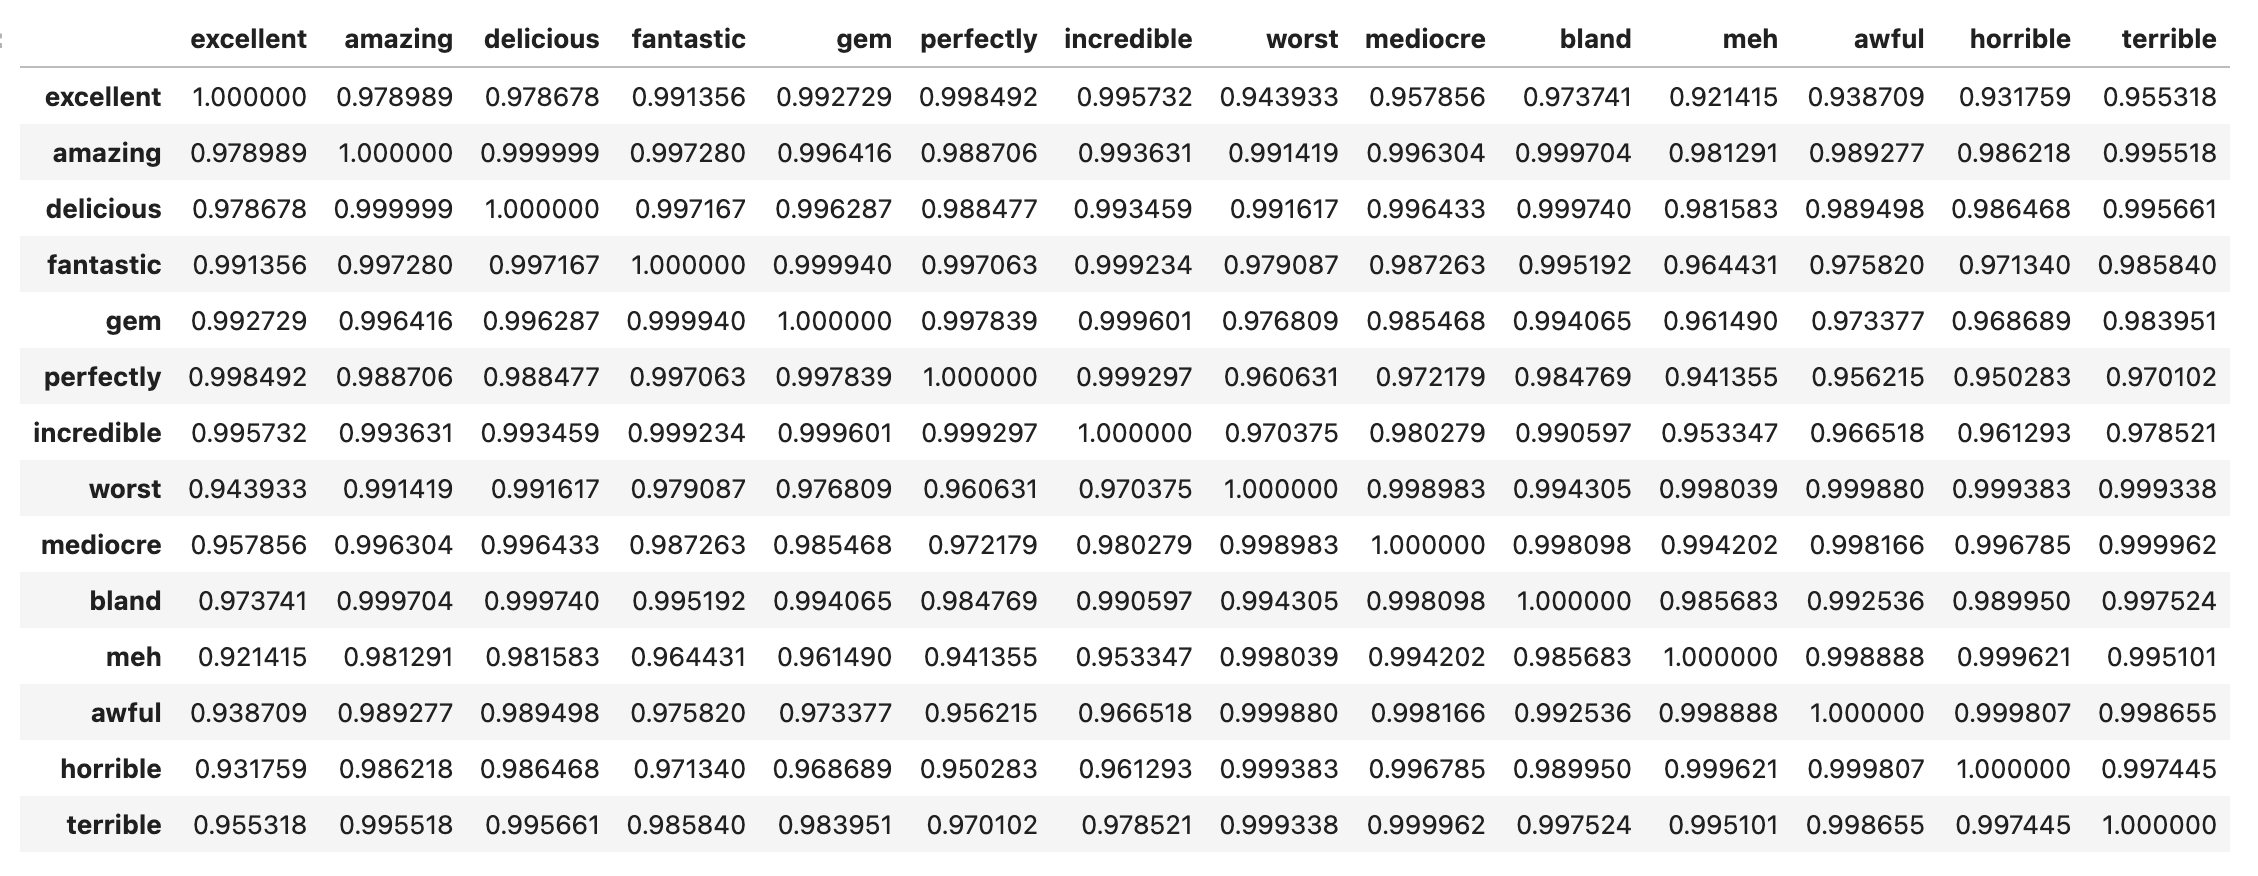
\includegraphics[scale=0.4]{images/5a.png}
    \caption{Table when $k=2$}
\end{figure}

\begin{figure}[H]
    \centering
    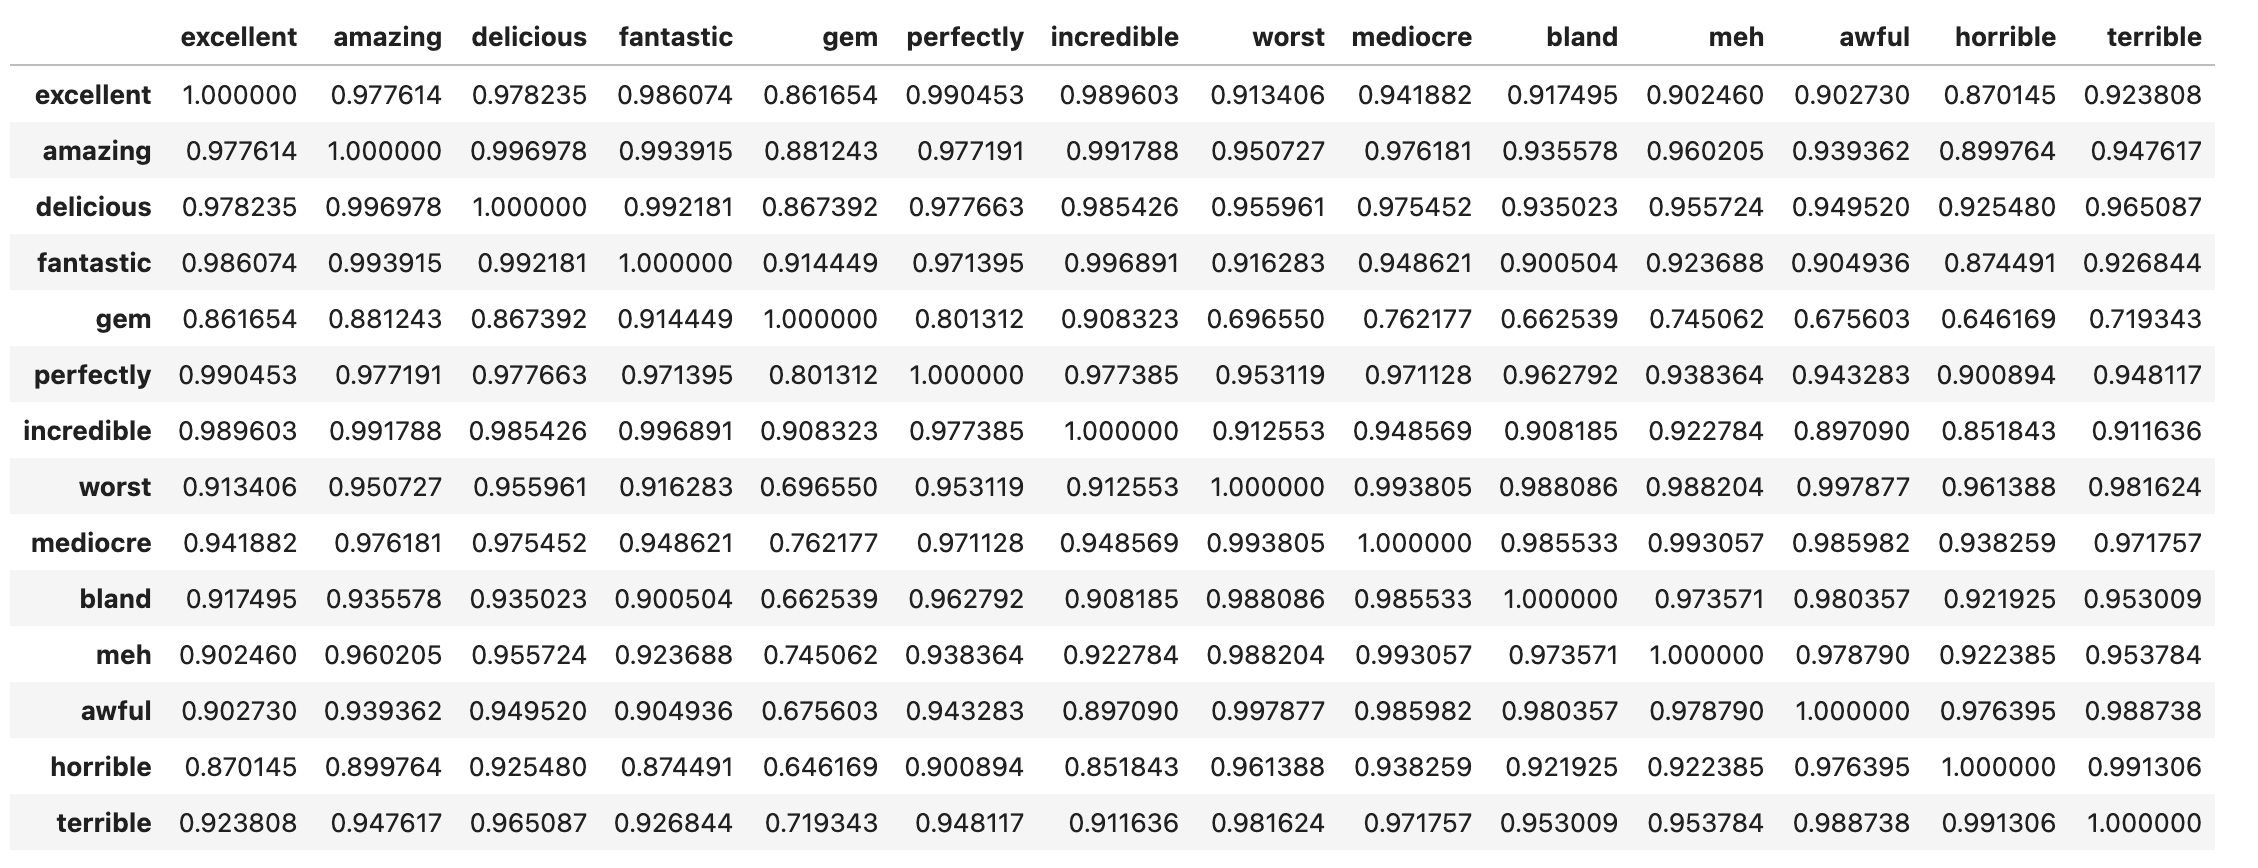
\includegraphics[scale=0.4]{images/5b.png}
    \caption{Table when $k=4$}
\end{figure}

\begin{figure}[H]
    \centering
    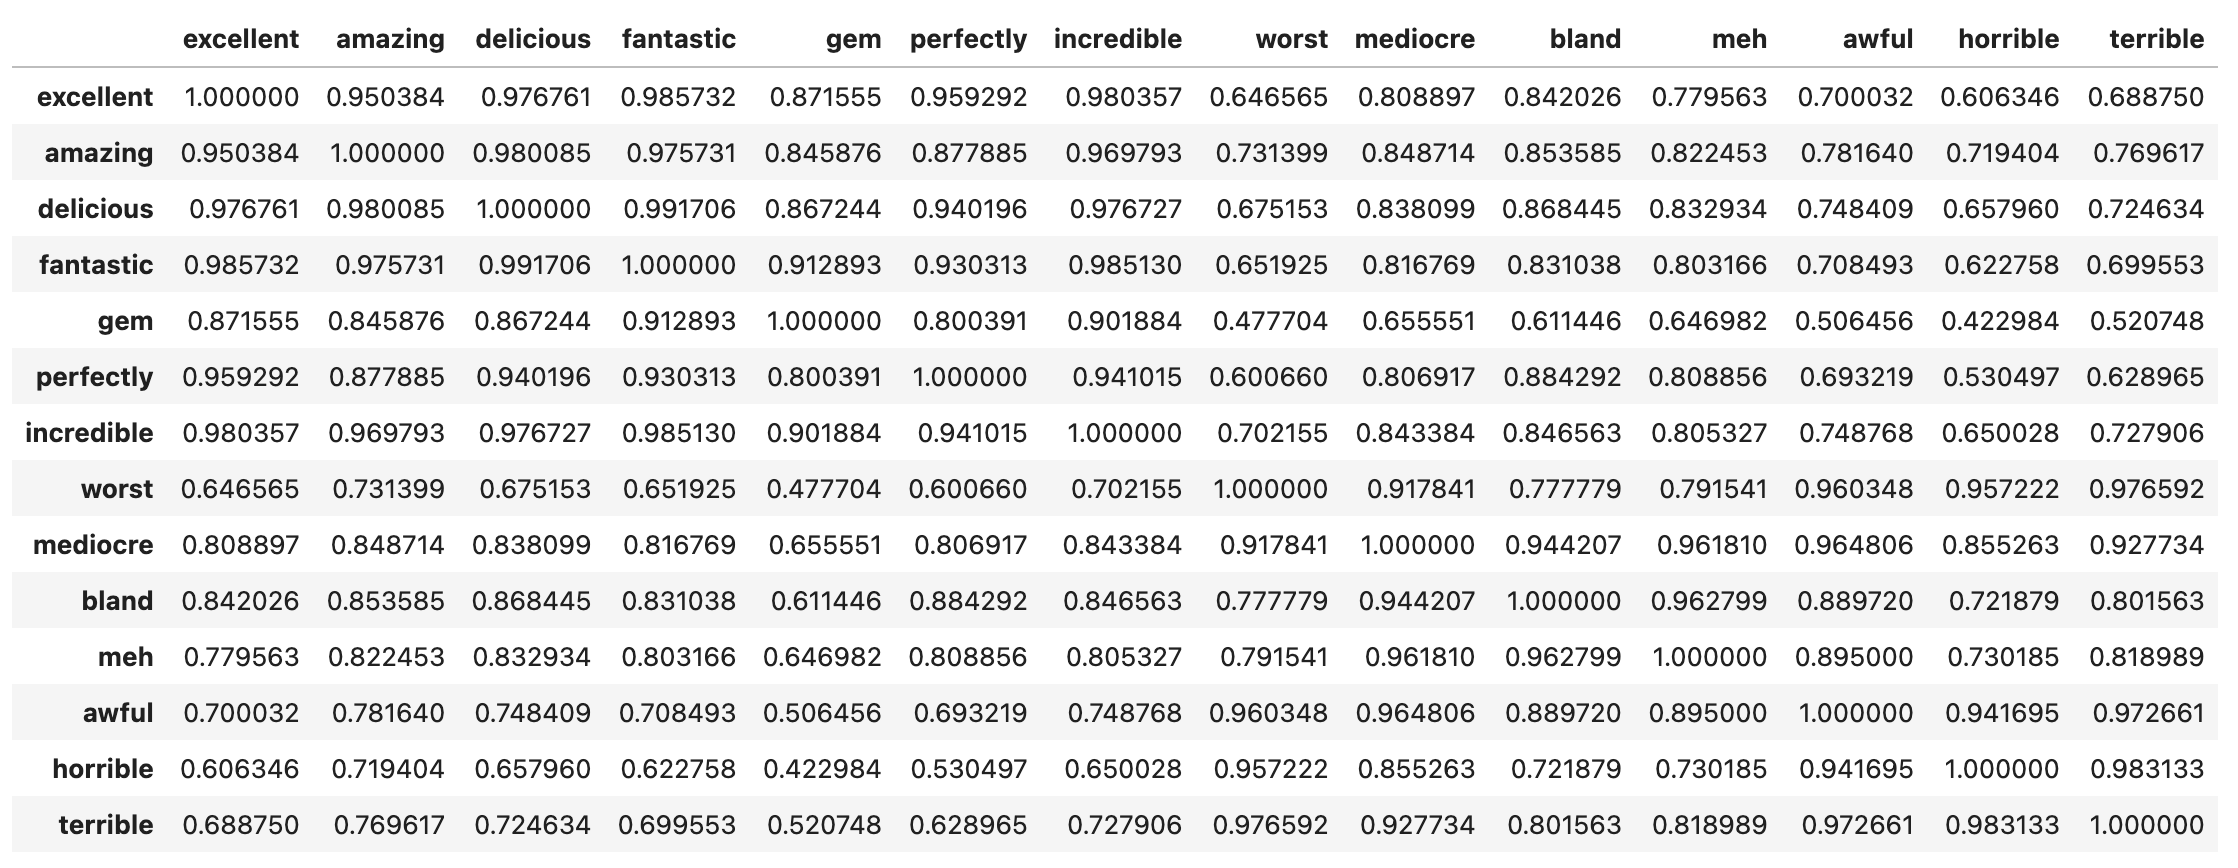
\includegraphics[scale=0.4]{images/5c.png}
    \caption{Table when $k=8$}
\end{figure}

\newpage
\section*{Problem 6}
\begin{figure}[H]
    \centering
    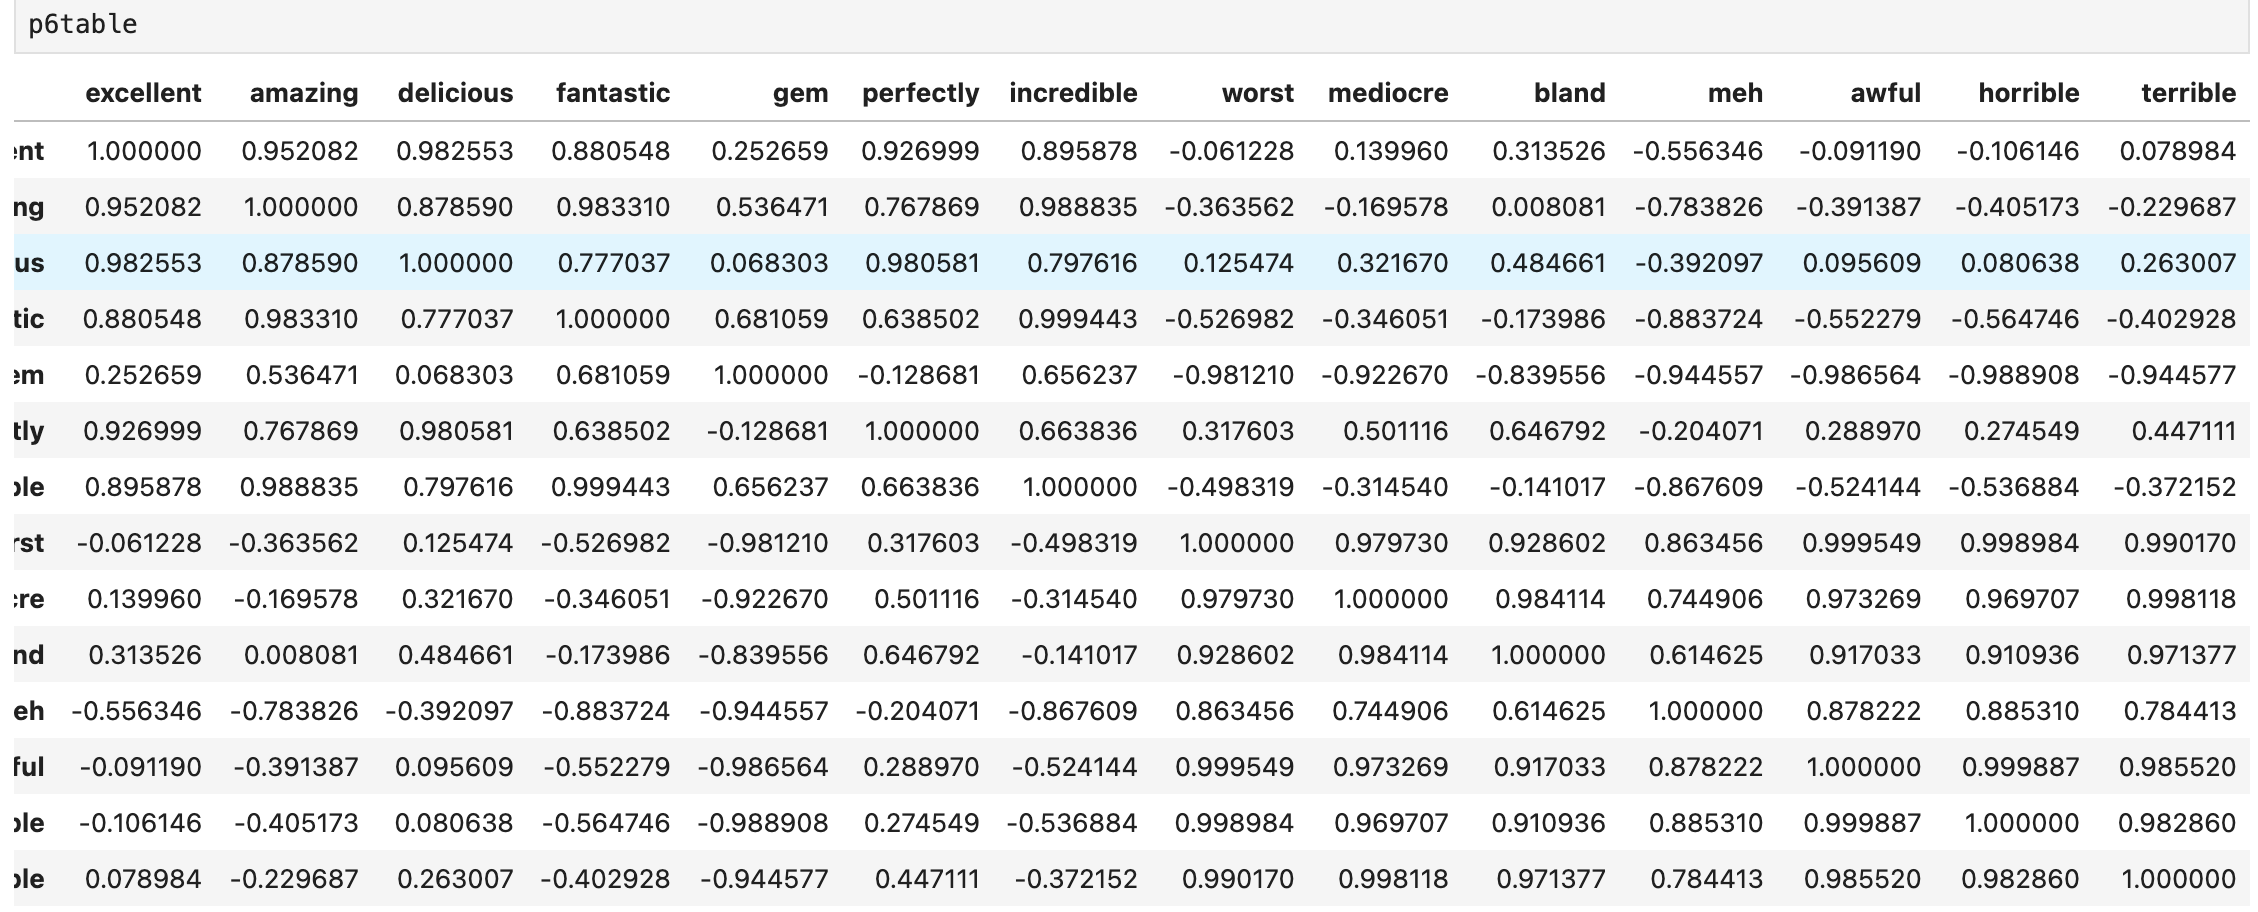
\includegraphics[scale=0.4]{images/6a.png}
    \caption{Table when $k=2$}
\end{figure}

\begin{figure}[H]
    \centering
    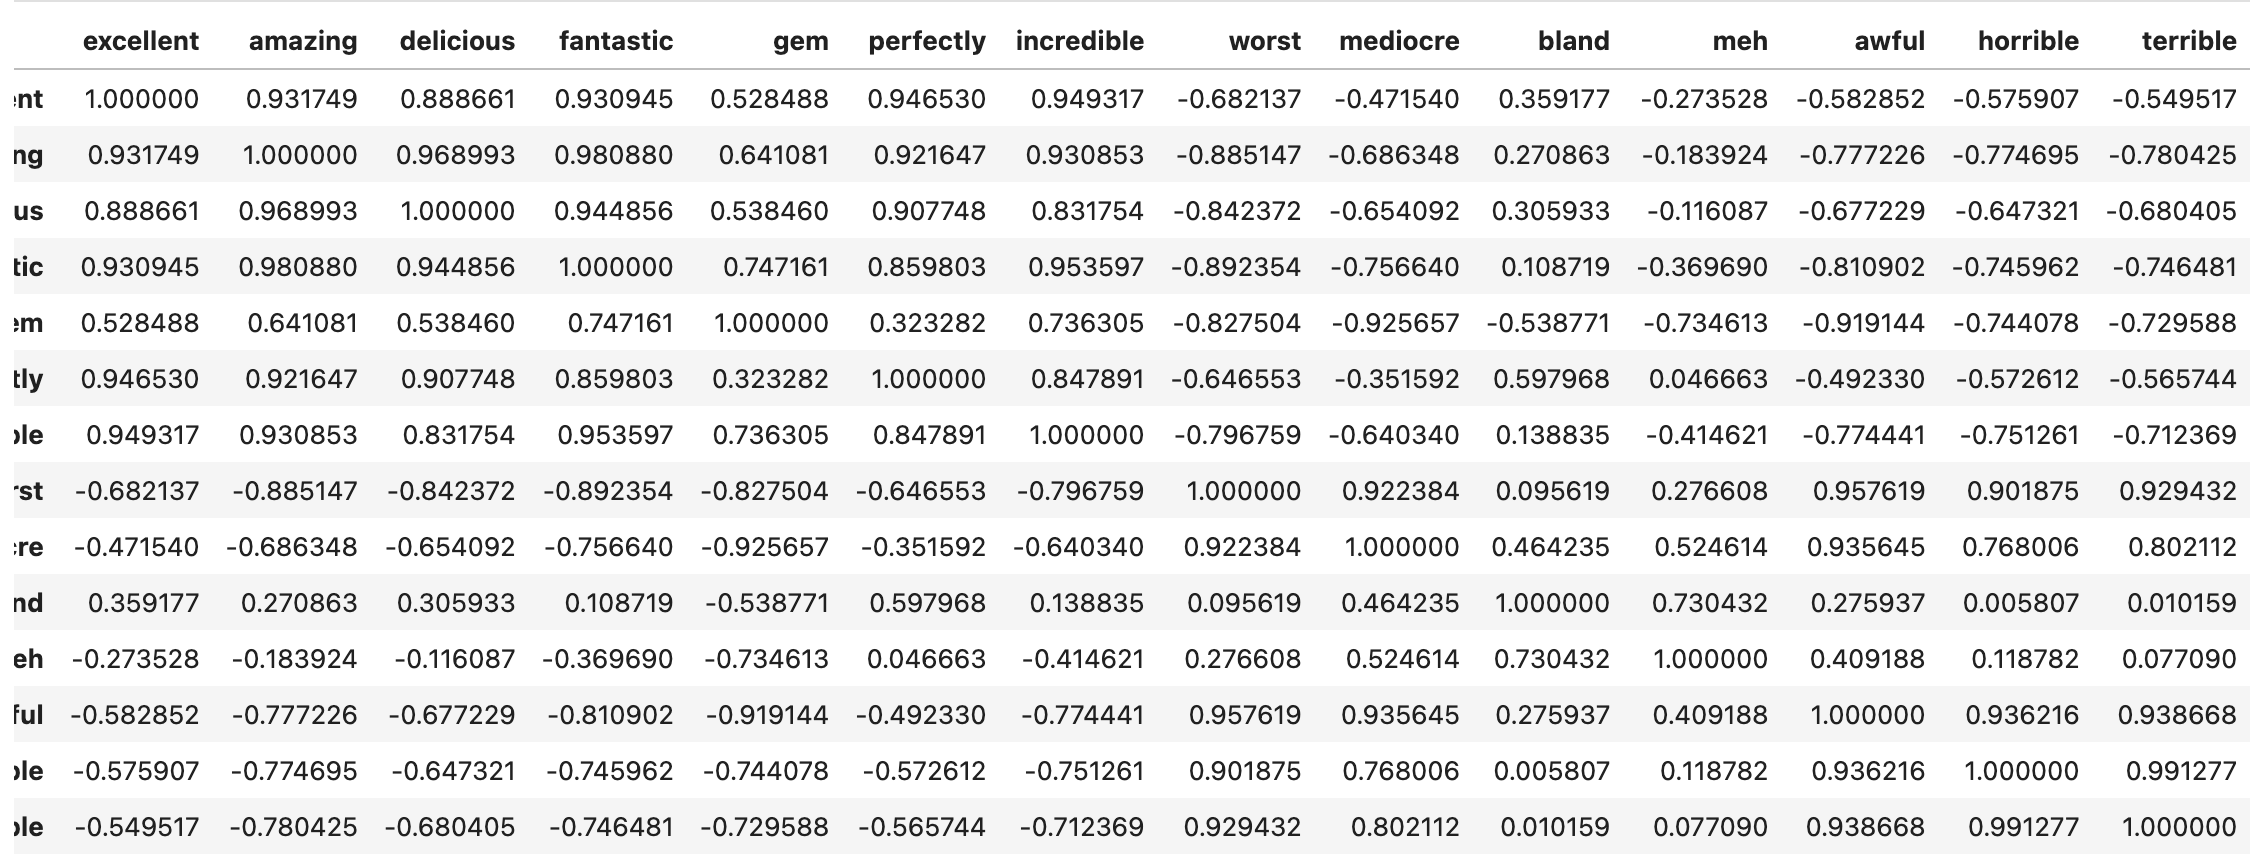
\includegraphics[scale=0.4]{images/6b.png}
    \caption{Table when $k=4$}
\end{figure}

\begin{figure}[H]
    \centering
    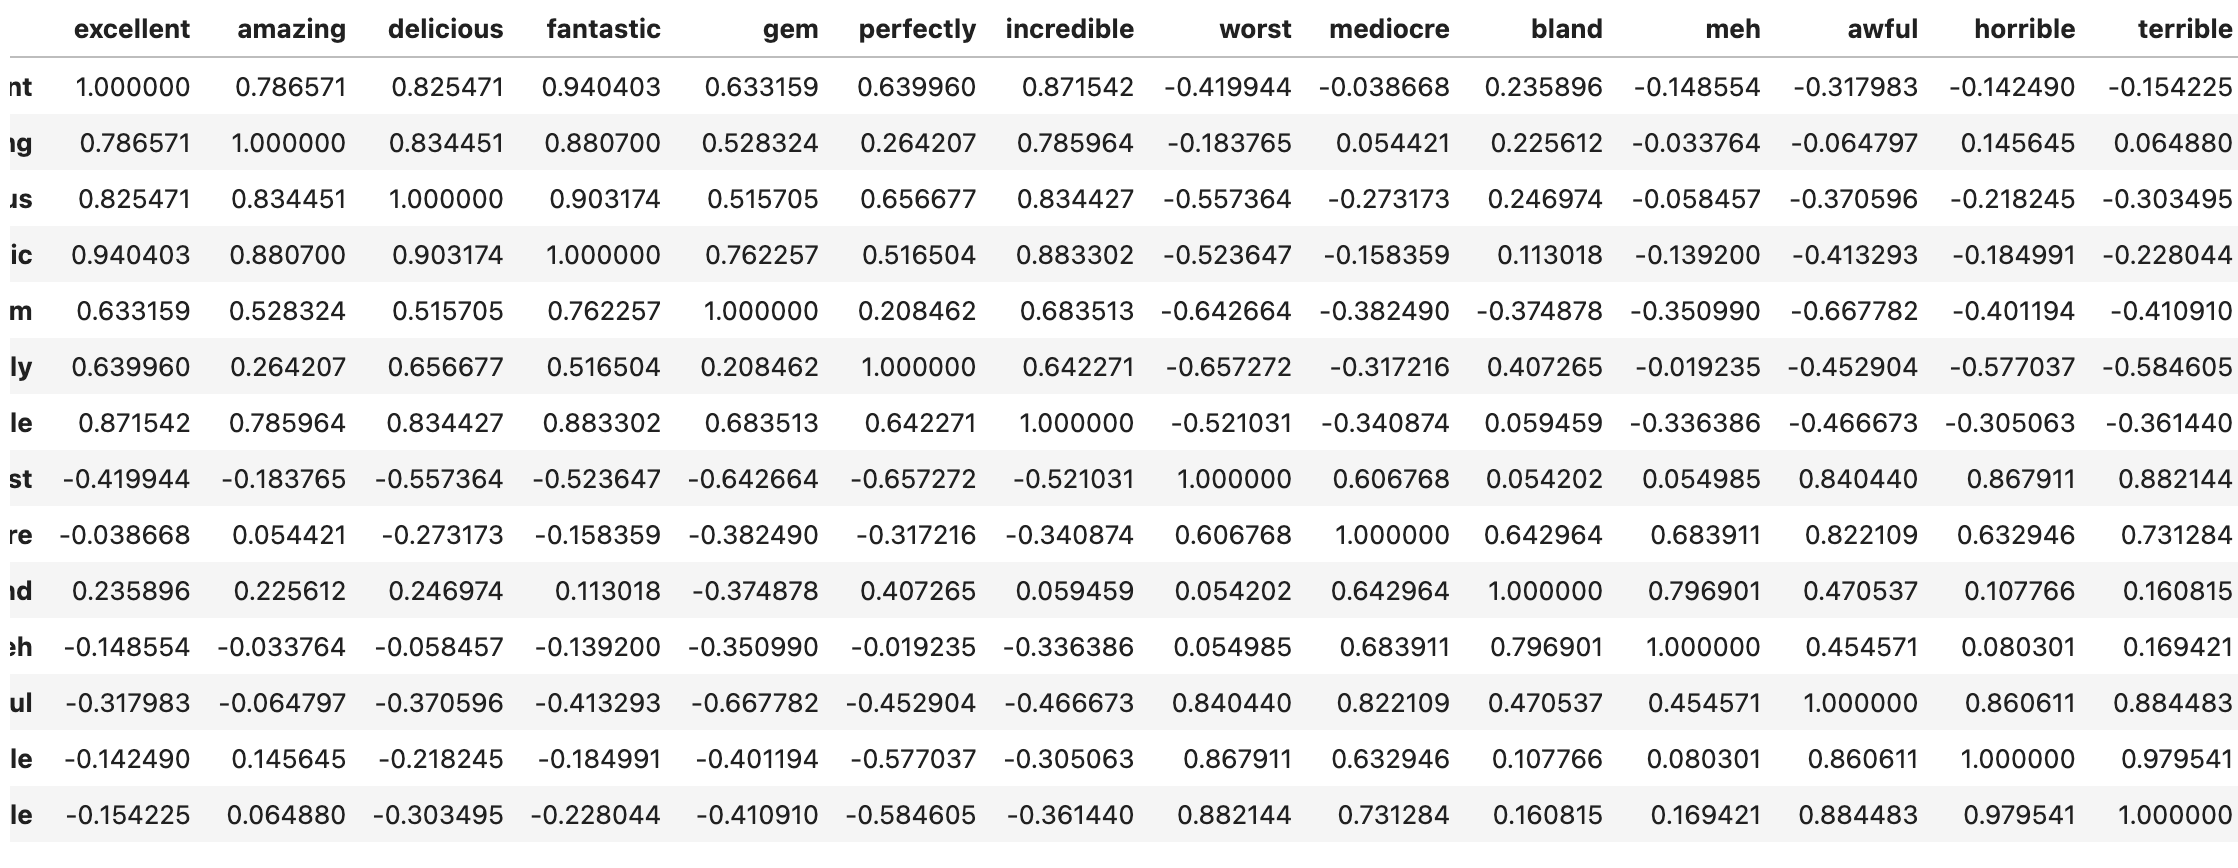
\includegraphics[scale=0.4]{images/6c.png}
    \caption{Table when $k=8$}
\end{figure}

\end{document}
